% Chapter 3

\chapter{Rigid Body Motion} % Main chapter title

\label{Chapter3} % For referencing the chapter elsewhere, use \ref{Chapter1} 

\lhead{Chapter 3. \emph{Rigid Body Motion}} % This is for the header on each page - perhaps a shortened title

%----------------------------------------------------------------------------------------

Previous chapters have disregarded rotational motion of solid bodies.  This chapters examines the mechanics of rigid body rotations and collisions through angular momentum fixed axis rotation.  Simulations will involve rigid body collisions.


\section{Angular Momentum and Torque}

Previous sections in this thesis have simply involved translational motion.  The theorem of rigid body motion states that the displacement of any rigid body can be decomposed into two independent motions: the translation of the center of mass, and the rotation about the center of mass.  A rigid body in general is defined as an object that maintains its shape and size when a force is applied to it.  In reality, all objects experience some level of deformation, however for the purpose of these simulations it is safe to ignore this.  

To rotate a rigid body about an axis, a force must be applied to create a moment of torque, given by the equation below:

\begin{equation} \label{eq:torquegeneral}
\vec{\tau} = \vec{r} \times \vec{F}
\end{equation}


Where $\vec{r}$ is the vector from center of rotation to the point of application of force.  If the force applied has a line of action that intersects the center of mass of the object, no torque is produced.  To simplify the simulations involving toruqe, all objects are polygons with an assumed uniform density.  Therefore, the center of mass would always be the geometric center of the polygon.  The center of mass is essential for simulations becuase it is the reference point that allows the simulations to involve both translational and rotational motion. 

While moment of torque represents resistance to angular motion, moment of inertia represents resistance to angular \textit{acceleration}.  For a continuous distribution of mass like a rigid body, the moment of intertia is defined by the following:

\begin{equation}\label{momentofintertia}
I =   \int  r^2 dm
\end{equation}

Lastly, while linear momentum is related to translational motion, angular momentum is related to rotational motion.  Angular momentum is defined by:  $\vec{L} = \vec{r} \times \vec{p}$.  A rigid body can be interpreted as a collection of particles all rotating with the same angular velocity $\omega$, which allows for the following equation:

\begin{equation}
L = \mathlarger{\mathlarger{\mathlarger{\Sigma}}} m_i r_i^2 \omega
\end{equation}

Using the definition of moment of inertia, the above equation can be written as:

\begin{equation}
\vec{L} = I \vec{\omega}
\end{equation}

Understanding these fundamental equations is the background for Newton's Second Law for rotational motion, which is essential for rigid body simulations.  Any rigid body can be visualized as a collection of infinitely small particles of mass $dm$, as shown below:

\begin{figure}[h] 
	\centering
		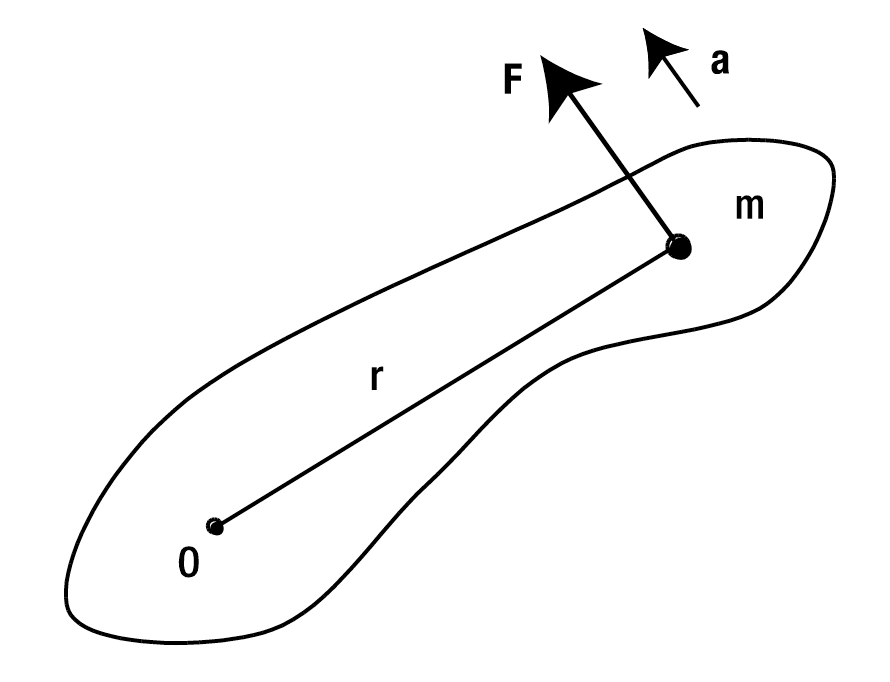
\includegraphics[width=7cm]{Figures/rigidbody.png}

	\caption{Diagram of rigid body with center of mass O}
	\label{fig:rigidbody}
\end{figure}

Understanding the equation $a = r \alpha$ and substituting into Newton's 2nd law yields the following:

\begin{equation}
F = mr\alpha
\end{equation}

Manipulating the scalar equation for torque of $T = Fr$ and combining with the above equation yields:

\begin{equation}
T = \mathlarger{\mathlarger{\mathlarger{\Sigma}}} m r^2 \alpha
\end{equation}

Again, understanding the equation for moment of inertia, and subsituting back for vectors yields the following:

\begin{equation}
\vec{T} = I \vec{\alpha}
\end{equation}

This formula is analagous to the common Newton's 2nd law of  $F = ma$ for rotational motion, instead of translational motion.  From this equation, the angular acceleration of any rigid body can be calculated from the torque, which is essential for creating simulations of rigid body rotation.  

\subsection{}













% \section{Rigid Body Collision}



